

\noindent \textbf{Coupled Multiscale Simulations}
The goal of this task is to investigate the use of Reduced Order Models (ROMs)
in combination with other computational fluid dynamics (CFD) and
thermal-hydraulic approaches to reduce computational cost. We note that ROMs
can be readily used in the context of systems analysis codes. We will
demonstrate this within the context of the recently developed SAM-NekRS
coupling in Cardinal.

ROMs can replace the solution of the Navier-Stokes equations with a simplified
model, which can greatly reduce computational time. However, some parts of the
domain may require additional resolution. Therefore, we will examine hybrid
LES-ROM models, which combine a ROM model for the entire system or assembly
with a localized, more detailed LES model for specific regions. An example for
a square bundle is shown in Fig.~\ref{fig:lesrom}, illustrating an example
of an assembly solved with a reduced order model, where four subchannels near a
thimble are solved with wall-resolved LES. Special attention needs to be paid
to the interface where unsteady Dirichlet conditions can be applied. The modal
decomposition of the reduced order model can reconstruct the flow field and
impose it as a boundary condition in the LES simulation.

For small LES domains, a one-way approach where information flows only from the
ROM to the LES may be sufficient. If the flow behavior within the LES domain is
expected to have a global impact, a two-way coupling approach is needed. We
will focus on an overlapping domain approach where the LES behavior is
translated into forcing terms for each mode of the ROM.

We will also examine RANS-ROM modeling as a potential interface for ROM
methods. This includes using previous work on rod bundles and sub-channels,
where high-fidelity simulation was used to improve RANS results
\cite{martinez2019a}.

Our aim is to develop a generalized interface between RANS and ROM. For
example, ROM results from one assembly can be superposed over a transient RANS
model of the entire system to recover unsteady features not modeled correctly
by RANS. To this end, it is crucial to ensure that the energy transfer between
scales is realistic. We will leverage recent work on the concept of a novel
energy-based ROM length scale \cite{mou2021}. We will also explore the
potential of an uplifting ROM approach \cite{ahmed2020} where closure and
projection errors are corrected in the prolongation to RANS.

\begin{figure}[t!] \centering
    {\setlength{\unitlength}{1.0in} \begin{picture}(6.5,2.500)(0.0,0)
      \put(0.9,-.10){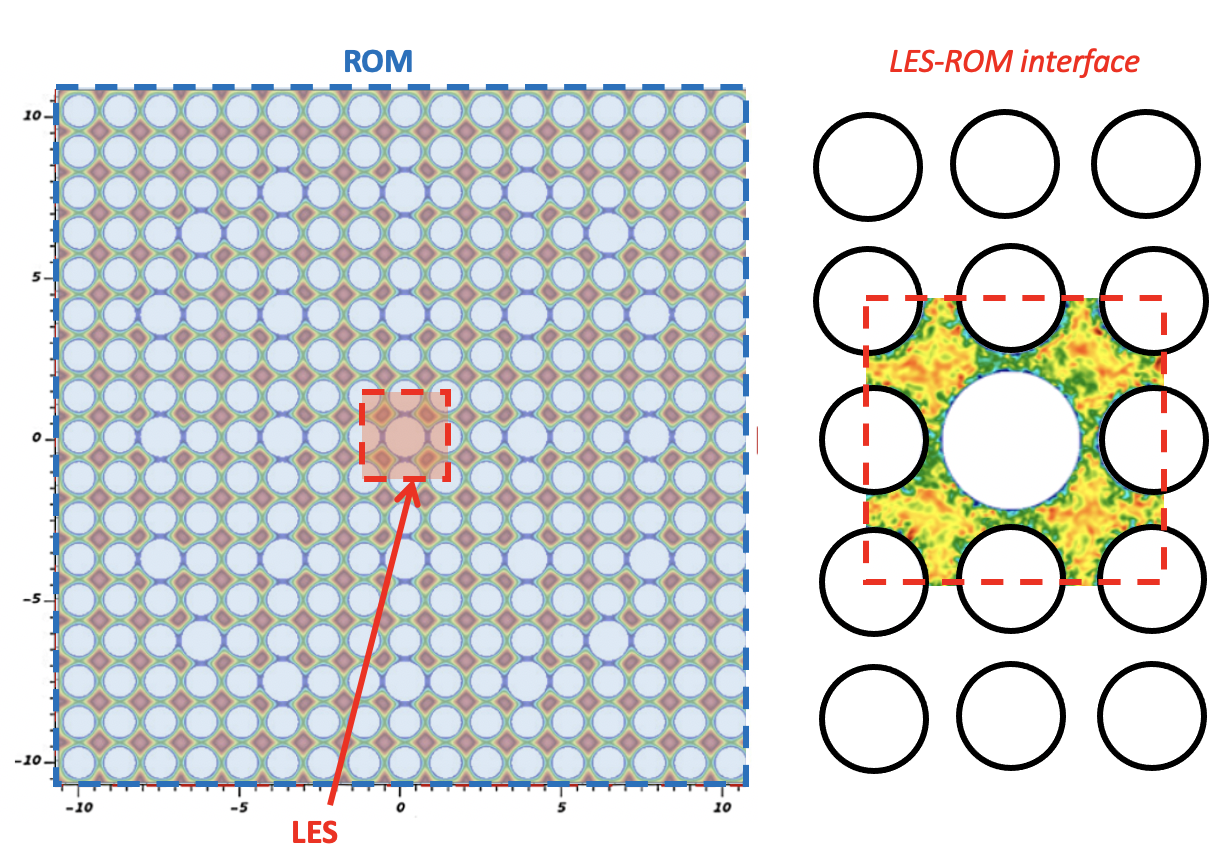
\includegraphics[height=2.7in]{figs/lesrom.png}}
    \end{picture}}
    \caption{Example of LES-ROM coupling \label{fig:lesrom}
\\[-3ex]
}
\end{figure}

